\paragraph{}En este proceso, el usuario administrador principal puede crear,
consultar, modificar o borrar centros de la aplicación.

\paragraph{}La figura \ref{diagramaNivel4-AdministrarCentros}
muestra el nivel de abstracción 4: Administrar centros.

  \begin{figure}[!ht]
    \begin{center}
      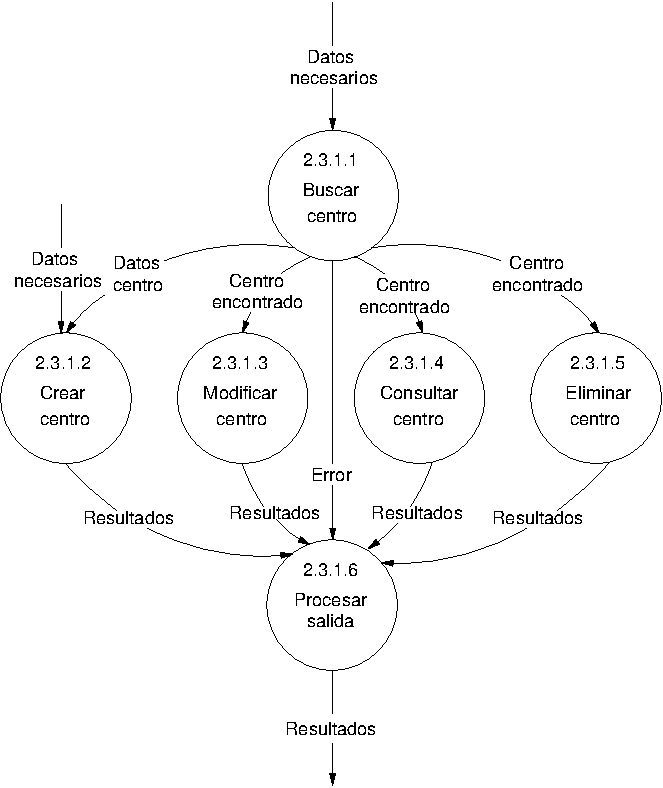
\includegraphics[]{08.Analisis_Funcional/8.2.DFDs/Niveles/Nivel4/AdministradorPrincipal/AdministrarCentros/Diagramas/nivel4-AdministrarCentros.pdf}
      \caption{Nivel de abstracción 4: Administrar centros.}
      \label{diagramaNivel4-AdministrarCentros}
    \end{center}
  \end{figure}
